\chapter{Evaluierung}\label{kap:eval}

Dieses Kapitel beschreibt die Auswertung der
Ergebnisse der trainierten Modelle.

Dafür werden im ersten Abschnitt zunächst die Metriken 
erklärt, anhand denen die Evaluierung erfolgte. 

Im zweiten Abschnitt werden die beiden verwendeten Model
Architekturen SSD und Fater R-CNN hinsichtlich dieser Metriken, sowie anhand 
inferenzergebnisse verglichen.

Der dritte Abschnitt beschreibt Methoden mit denen 
die Ergebnisse das Faster R-CNN optimiert werden konnten und im 
vierten Abschnitt werden die Modelle noch einmal miteinander
verglichen, dieses mal hinsichtlich der Inferenzzeit.

\section{Evaluierungs Metriken}\label{sec:metricen}

\subsection*{Mean Average Precision (mAP)}

Zur Messung der Genauigkeit der Object Detection Modelle 
wurde die \textit{Mean Average Precision (mAP)} verwendet.

Diese bezieht sowohl Klassifizierungs- als auch Lokalisierungsgenauigkeit 
mit ein und lässt sich aus den folgenden Werten errechnen.

\begin{itemize}
  \item \textit{True Positive (TP)}: Das Model hat richtig das Vorhandensein eines Objekts geschätzt
  \item \textit{True Negative (TN)}: Das Model hat richtig die Abwesenheit eines Objekts geschätzt
  \item \textit{False Positive (FP)}: Das Model hat fälschlicherweise das Vorhandensein eines Objekts geschätzt
  \item \textit{False Negative (FN)}: Das Model hat fälschlicherweise die Abwesenheit eines Objekts geschätzt
\end{itemize}

Die festlegung, für True Positive Werte wird dabei über die 
Intersection over Union ermittelt.

Diese ist durch den Überlappungsgrad der gelabelten (Ground Truth) und der
geschätzete Boundig Box zu dem Gesammtbereich 
beider Boxen definiert.

Beträgt dieser mehr als ein bestimmter Threshhold, häufig 50\%,
gilt die Schätzung als \textit{True Positive}, andernfalls als 
\textit{False Positive}. 


\newcommand\MyBox[2]{
  \fbox{\lower0.75cm
    \vbox to 1.7cm{\vfil
      \hbox to 1.7cm{\hfil\parbox{1.4cm}{#1\\#2}\hfil}
      \vfil}%
  }%
}
\noindent
\renewcommand\arraystretch{1.5}
\setlength\tabcolsep{0pt}

\begin{minipage}{\textwidth}
    \begin{minipage}[b]{0.49\textwidth}
      \centering
      \def\svgwidth{0.8\textwidth}
      \input{Bilder/IoU_formula.pdf_tex}
      \captionof{figure}{Intersection over Union}
      \label{fig:iou}
  \end{minipage}
    \hfill
    \begin{minipage}[b]{0.49\textwidth}
      \centering
      \begin{tabular}{c >{\bfseries}r @{\hspace{0.7em}}c @{\hspace{0.4em}}c @{\hspace{0.7em}}l}
        \multirow{10}{*}{\rotatebox{90}{\parbox{2.5cm}{\bfseries\centering Tatsächlicher Wert}}} & 
          & \multicolumn{2}{c}{\bfseries Geschätzter Wert} & \\
        & & \bfseries p & \bfseries n & \bfseries\\
        & p$'$ & \MyBox{True}{Positive} & \MyBox{False}{Negative}\\[2.4em]
        & n$'$ & \MyBox{False}{Positive} & \MyBox{True}{Negative} \\
      \end{tabular}
        \captionof{figure}{Confusion Matrix}
        \label{fig:confusion_matrix}
    \end{minipage}
\end{minipage}

\vspace{1cm}

Anhand dieser, in der Confusion Matrix dargestellen, Werte 
lassen sich \textit{Precision} und \textit{Recall} berechnen.

Dabei ist der Recall definiert durch das Verhältniss der
richtig gefundenen zu allen im Bild befindlichen Objekten, 
oder anders ausgedrück die True Positives zu True Positive + 
False Negatives wie in Geichung \ref{eq:recall} dargestellt.

\begin{equation}
  \label{eq:recall}
  Recall = \frac{TP}{TP + FN}
\end{equation}

\vspace{0.5cm}

Im Gegensatz zu Recall welcher die Trefferquote angibt, 
gibt die Precision die Genauigkeit an mit der die Objekte
gefunden werden.

Die Precision ist durch das Verhältnis der Richtigen 
Schätzungen bezogen auf alle gemachten Schätzungen definiert, 
was durch die True Positives durch die True Positives + 
False Positives wie in Gleichung \ref{eq:precision}
dargestellt ausgedrückt wird.


\begin{equation}
  \label{eq:precision}
  Precision = \frac{TP}{TP + FP}
\end{equation}

\vspace{0.5cm}

Stellt man den Recall, welcher die Trefferquote angibt, und der 
Precision welche die Genauigkeit der treffer angibt gemeinsam 
dar ergibt sich die \textit{Precision-Recall-Kurve}, dessen 
Fläche die \textit{Average Prcision} für eine klasse darstellt.
Für alle Klassen im Mittel ergibt sich so die \textit{mean Average 
Precision}.

\vspace{0.5cm}

\begin{equation}
  Average Precision = \sum(Precision(Recall))
\end{equation}

\begin{equation}
  mAP = \frac{1}{N} \sum AP
\end{equation}

\vspace{0.5cm}





\subsection*{Fehlerfunktion (Loss)}
Die Fehlerfunktion setzet sich aus einem Lokalisierungs- und einem 
Klassifikationsfehler zusammen. 
Die Lokalisierung erfolgt über eine Lineare Regression zur 
Annäherung der Bounding Boxes and die richtigen Koordinaten.



%----------------- SECTION: validtaion ---------------------
\section{Vergleich der Modelle}\label{sec:model_vergleich}

Dieser Abschnitt beschreibt, wie die beiden für das Training 
verwendeten Object Detection Architekturen Single Shot Detector (SSD)
und Faster R-CNN mit verschiedenen basis
CNNs und Datensatzaufbereitungen miteinander verglichen und 
ausgewertet wurden.


\subsection{Evaluierung/Validierung}

Die im Folgenden dargestellte Ergebnisse beziehen sich auf 
den Validierungsanteil des für das Training verwendeten 
OpenImages Datensatzes.

Die Berechnung anhand der in Abschnitt \ref{sec:metricen}
 erläuterten 
Metriken konnte dabei mithilfe Tensorflow durchgeführt 
und während des Trainings mit in dem Evaluierungs-Tool 
Tensorboard visualisiert werden.

Der Single Shot Detector wurde mit den Basis CNNs MobilenetV2 und
InceptionV2 trainiert, das Faster R-CNN nur mit dem InceptionV2.
Dabei wurden jeweils einmal der augmentierte une einmal 
der originale Datensatz verwendet.


% SSD wurd mit Batchsize=12 75k durchläufe trainiert.\\
% Faster R-CNN mit Batchsize=1 für 200k durchläufe.(1 weil dynamische input size)\\
% eine epoche sind (teps mal batchsize)/samples
\vspace{0.5cm}
\begin{table}[H]
  \centering
  \begin{tabular}{m{0.25\textwidth}m{0.2\textwidth}|m{0.15\textwidth}<{\centering}m{0.15\textwidth}<{\centering}}
  \hline
  Model                                                              & Optimierung                                                                   & mAP                                                        & Loss                                                       \\ \hline\hline
  SSD + MobilenetV2                                                  & \begin{tabular}[c]{@{}l@{}}Ohne\\ Augmentierung\end{tabular}                  & \begin{tabular}[c]{@{}l@{}}0,62\\ 0,61\end{tabular}        & \begin{tabular}[c]{@{}l@{}}3,56\\ 3,50\end{tabular}        \\ \hline
  SSD + InceptionV2                                                  & \begin{tabular}[c]{@{}l@{}}Ohne\\ Augmentierung\end{tabular}                  & \begin{tabular}[c]{@{}l@{}}0,65\\ 0,62\end{tabular}        & \begin{tabular}[c]{@{}l@{}}3,86\\ 3,71\end{tabular}        \\ \hline
  \begin{tabular}[c]{@{}l@{}}Faster R-CNN\\ +InceptionV2\end{tabular} & \begin{tabular}[c]{@{}l@{}}Ohne\\ Augmentierung\\ Early Stopping\end{tabular} & \begin{tabular}[c]{@{}l@{}}0,67\\ 0,69\\ 0,67\end{tabular} & \begin{tabular}[c]{@{}l@{}}0,82\\ 0,67\\ 0,69\end{tabular} \\ \hline
  \end{tabular}
  \caption{}
  \label{table:model_vgl}
\end{table}
\vspace{0.5cm}

Anhand der in Tabelle \ref{table:model_vgl} dargestellten 
Ergebnisse ist zu erkennen, das sich mit der zweistufigen 
Model Architekur des Faster R-CNN bessere Ergebnisse als mit 
dem einstufigen SSD erzielen ließen. Dieser war besonders 
deutich anhand der Loss Werte festzustellen.

Desweiteren werden unter den SSD Konfigurationen mit dem InceptionV2 
als Basis CNN bessere Ergebnisse als mit dem weniger komplexen 
MobilenetV2 erreicht.

Bei allen Modellen war durch die Augmentierung eine Verbesserung 
des Loss Wertes festzustellen.

Bei den Varianten mit der SSD Architektur führt die Augmentierung
jedoch auch zu einer verringerung des mAP Wertes, 
was auf die weniger komplexe Model Struktur zurückzuführen sein kann.

Je mehr Parameter einem Model zu verfügung stehen, desto besser kann 
es sich an die Trainingsdaten anpassen, desto eher findet jedoch
auch eine Überanpassung (Overfitting) statt, was hier bei dem 
komplexeren Faster R-CNN Modell zu beobachten ist.

Der Plot in Abbildung \ref{plot:loss} zeigt den Trainingsverlauf 
der Faster R-CNN Trainingskonfigurationen anhand der Losskurve.

Für das Training mit dem Original Datensatz nimmt diese ab ca.
100k Iterationen wieder zu, wohingegen der Loss beim Training 
mit augmentierten Datensatz den Wert relativ beibehalten 
kann.

Early Stopping war, beim Faster R-CNN Modell, ein weiter Ansatz 
Overfitting zu vermeiden. Dabei wird, bevor der Loss Wert anfängt
sich wieder zu verschlechtern, das Training abgebrochen.

Anhand der Losskurve \ref{plot:loss} ist zu erkennen, dass sich
dadurch die gleichen Werte wie durch Augmentierung erreichen ließ.
Auf der anderen Seite kann der mAP Wert, wie in Abblidung \ref{plot:mAP}
zu erkennen ist durch das frühzeitige Stoppen seinen Endwert nicht 
erreichen.

\vspace{0.5cm}
\begin{figure}[H]
\begin{minipage}{0.5\textwidth}
  \centering
  \def\svgwidth{0.95\textwidth}
  \input{Bilder/plots/overfitting_kein_early_aug_mAP.pdf_tex}
  \captionof{figure}{mAP}
  \label{plot:mAP}
\end{minipage}
\begin{minipage}{0.5\textwidth}
  \centering
  \def\svgwidth{0.95\textwidth}
  \input{Bilder/plots/overfitting_kein_early_aug_loss.pdf_tex}
  \captionof{figure}{Loss}
  \label{plot:loss}
\end{minipage}
\end{figure}

% Legende: Overfitting
\begin{table}[htb]
  \centering
  \begin{tabular}{m{0.1\textwidth}<{\centering}m{0.2\textwidth}<{\centering}m{0.2\textwidth}<{\centering}}
    $\color[HTML]{FF7043}\medbullet$  Ohne & $\color[HTML]{0077BB}\medbullet$  Early Stopping & $\color[HTML]{CC3311}\medbullet$  Augmentierung
  \end{tabular}    
\end{table}

% colors
% orange: FF7043
% blue  : 0077BB
% red   : CC3311

Daraus lässt sich schließen, dass Augmentierung das 
bessere Verfahren gegen Overfitting ist. Um herauszufinden 
ob sich die Vermutung bestätigen lässt und wie sehr sich 
die Unterschiedlichen Ergebnisse zwischen SSD und 
Faster R-CNN in der Praktischen Anwendung bemerkbar 
machen wurde die Inferenz der Trainierten Modelle auf 
verschiedene Biler testweise ausgeführt.




%----------------- SECTION: Test Inferenz ---------------------
\subsection{Test Inferenz}\label{sec:test_inferenz}

Um die Inferenz testweise für verschiedene Bilder ausführen zu 
können wurden die trainierten Modelle wie in \ref{sec:inferenz}
beschrieben zunächst mithilfe des Model Optimizers in die 
\textit{Intermediat Representation (IR)} und anschlieoßen 
mit der Inferenz Engine in einem Python Script zur 
inferenz auf den NCS2 geladen.

Mithilfe des Scripts wurde dann die Inferenz für die 
verschiedenen Model- und Datensatzkonfigurationen
zunächst auf den Testanteil des für das Trainng verwendeten 
OpenImages Datensatzes ausgeführt.
Da dieser recht ähnlich zum Trainingsdatensatz ist 
wurden, um die Robustheit der Modelle gegenüber anderen 
Daten testen zu können, die Inferenz zum einen auf selbst
aufgenommene Bilder und zum anderen auf einen neuen Datensatz,
dem \textit{iWildCam 2019 Dataset} \cite{beery2019iwildcam}
ausgeführt. Dabei wurden nur die auf augmentierte Daten trainierten 
Modelle berücksichtigt. 




\subsubsection{OpenImages Test Set}

Die Inferenzergebnisse des OpenImages Test Sets 
ergaben, das in den meisten Fällen sowohl das SSD
als auch das Faster R-CNN die Tiere in den Bildern 
richtig erkannten.

Waren die Tiere jedoch sehr weit weg, mehrere gleichzeitig im Bild 
oder mit schlechter Qualität abgebildet,
vielen die Ergebnisse beim Faster R-CNN besser aus, wie in 
den Abbilungen \ref{fig:infer_res_ssd} und \ref{fig:infer_res_faster_rcnn}
zu erkennen ist.
Der Unterschied zwischen MobilenetV2 und InceptionV2 beim SSD 
sowie zwischen Early Stopping und Augmentierung beim Faster R-CNN 
war nur sehr gering.

\vspace{1cm}


\begin{minipage}{0.5\textwidth}
  \centering
  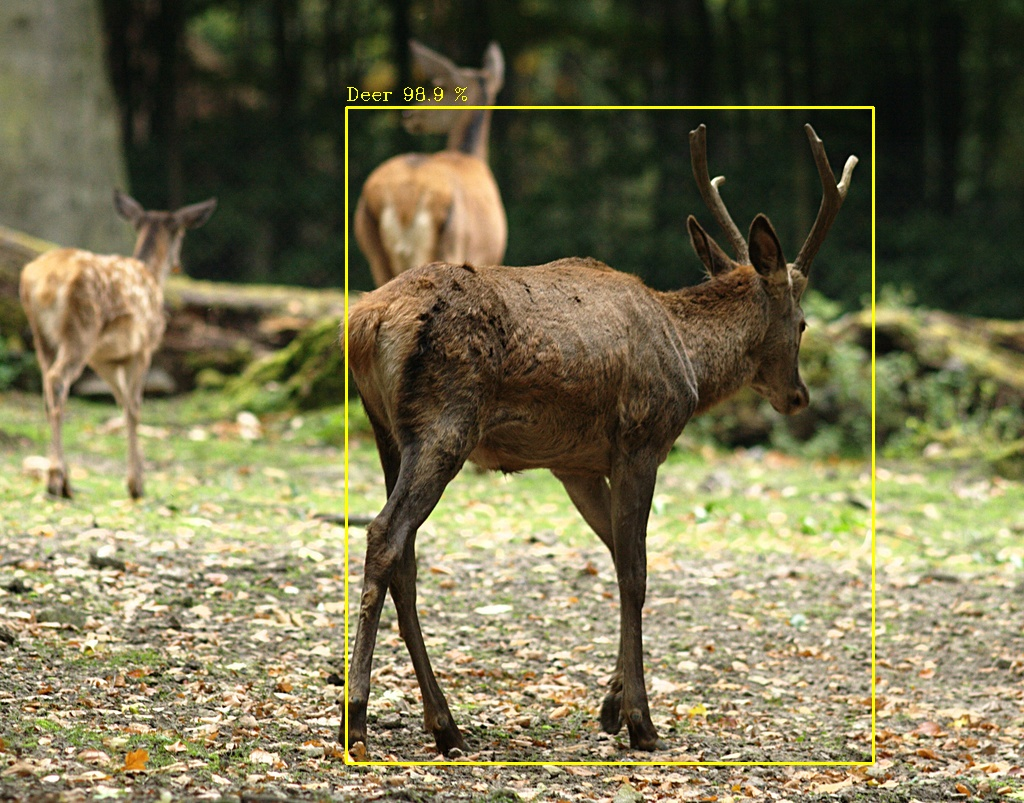
\includegraphics[width=0.9\textwidth]{model_compare_test__ssd_inception_v2.jpg}
  \captionof{figure}{SSD}
  \label{fig:infer_res_ssd}
\end{minipage}
\begin{minipage}{0.5\textwidth}
  \centering
  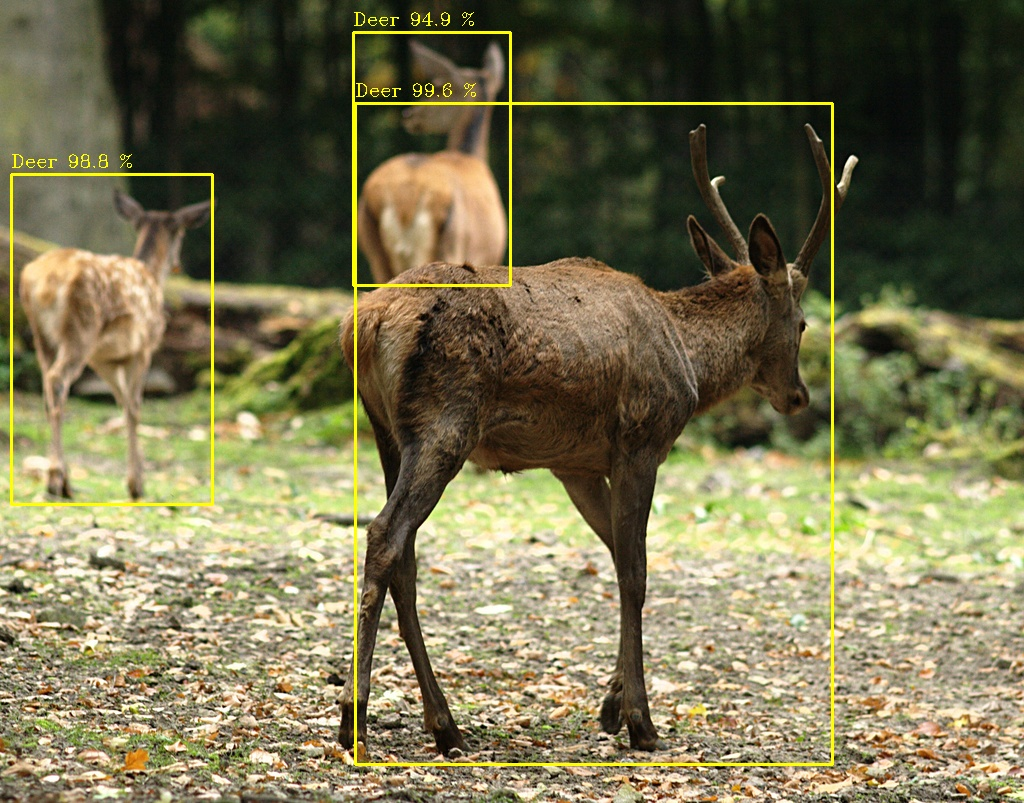
\includegraphics[width=0.9\textwidth]{model_compare_test__faster_rcnn_inception_v2_early_stopping.jpg}
  \captionof{figure}{Faster R-CNN}
  \label{fig:infer_res_faster_rcnn}
\end{minipage}


\subsubsection{Eigene Aufnahmen}

Bei der Inferenz auf die eigenen Bilder 
war ein deutlicher Unterschied der Modell festzustellen.
In aufsteigender Reihenfolge lieferten SSD + MobilenetV2,
SSD + InceptionV2, Faster R-CNN mit 
Early Stopping und Faster R-CNN mit Augmentierten Daten
wie in den Abbildungen \ref{fig:infer_res_ssd_mobile}
bis \ref{fig:infer_rest_rcnn_aug} festzustellen ist, 
bessere Ergebnisse.


\vspace{1cm}
\begin{minipage}{0.5\textwidth}
  \centering
  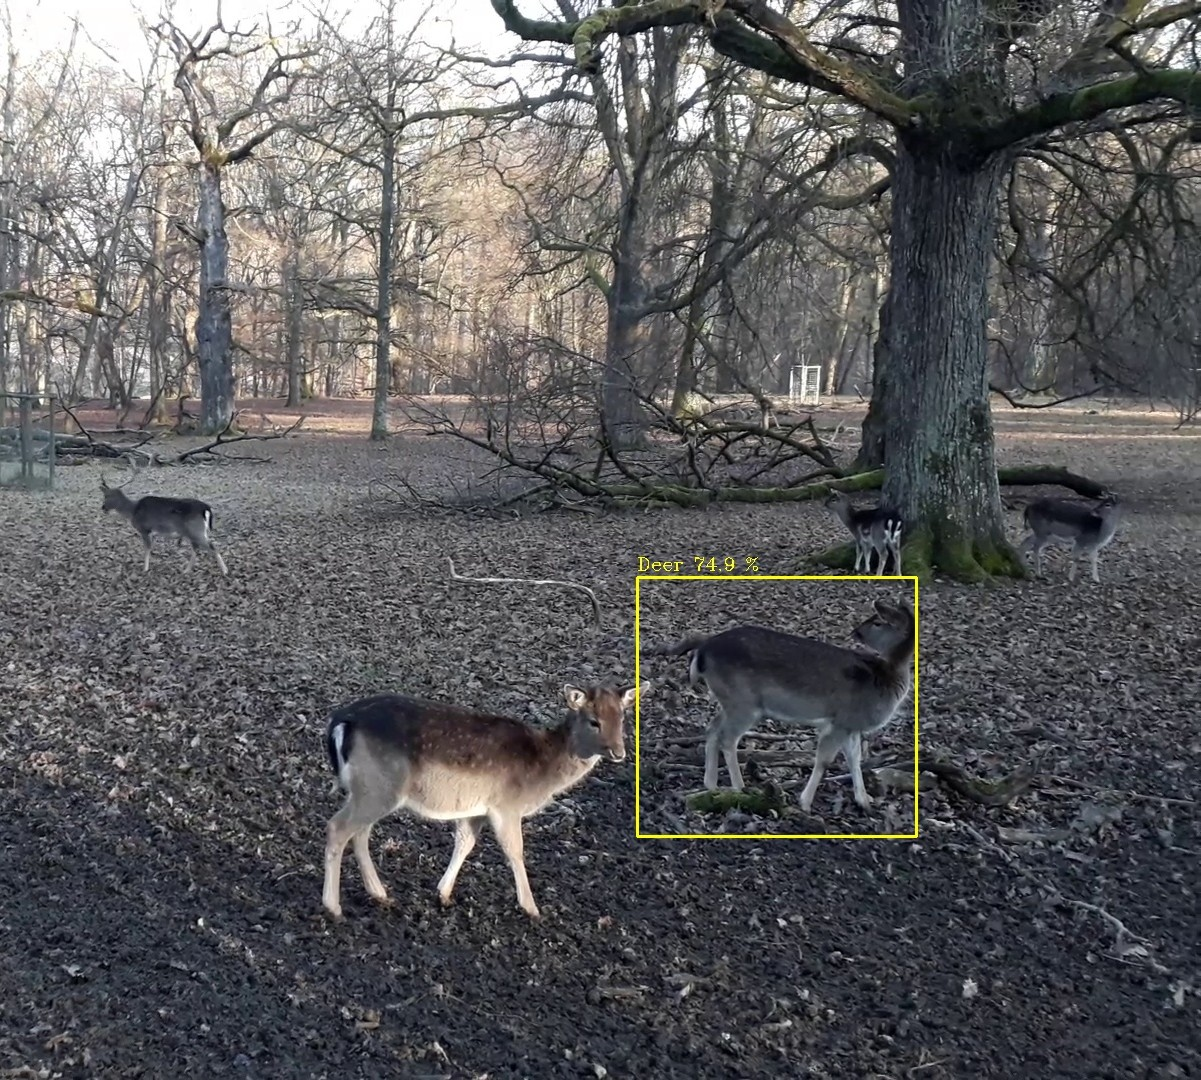
\includegraphics[width=0.9\textwidth]{model_compare_handy_ssd_mobilenet_v2.jpg}
  \captionof{figure}{SSD Mobilnet}
  \label{fig:infer_res_ssd_mobile}
\end{minipage}
\begin{minipage}{0.5\textwidth}
  \centering
  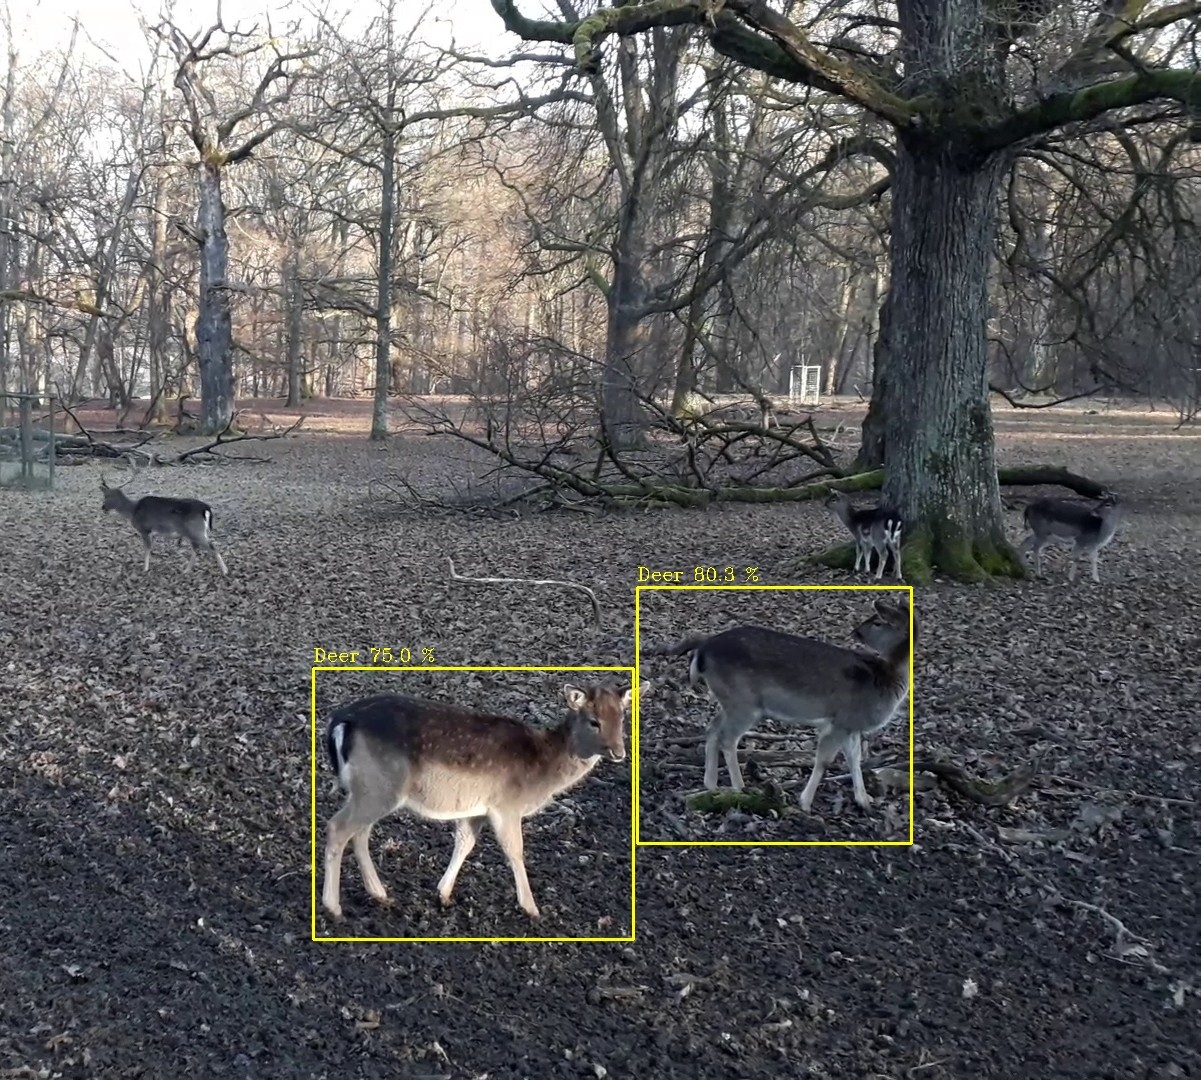
\includegraphics[width=0.9\textwidth]{model_compare_handy_ssd_inception_v2.jpg}
  \captionof{figure}{SSD Inception}
  \label{fig:infer_res_ssd_inception}
\end{minipage}
\\[1cm]
\begin{minipage}{0.5\textwidth}
  \centering
  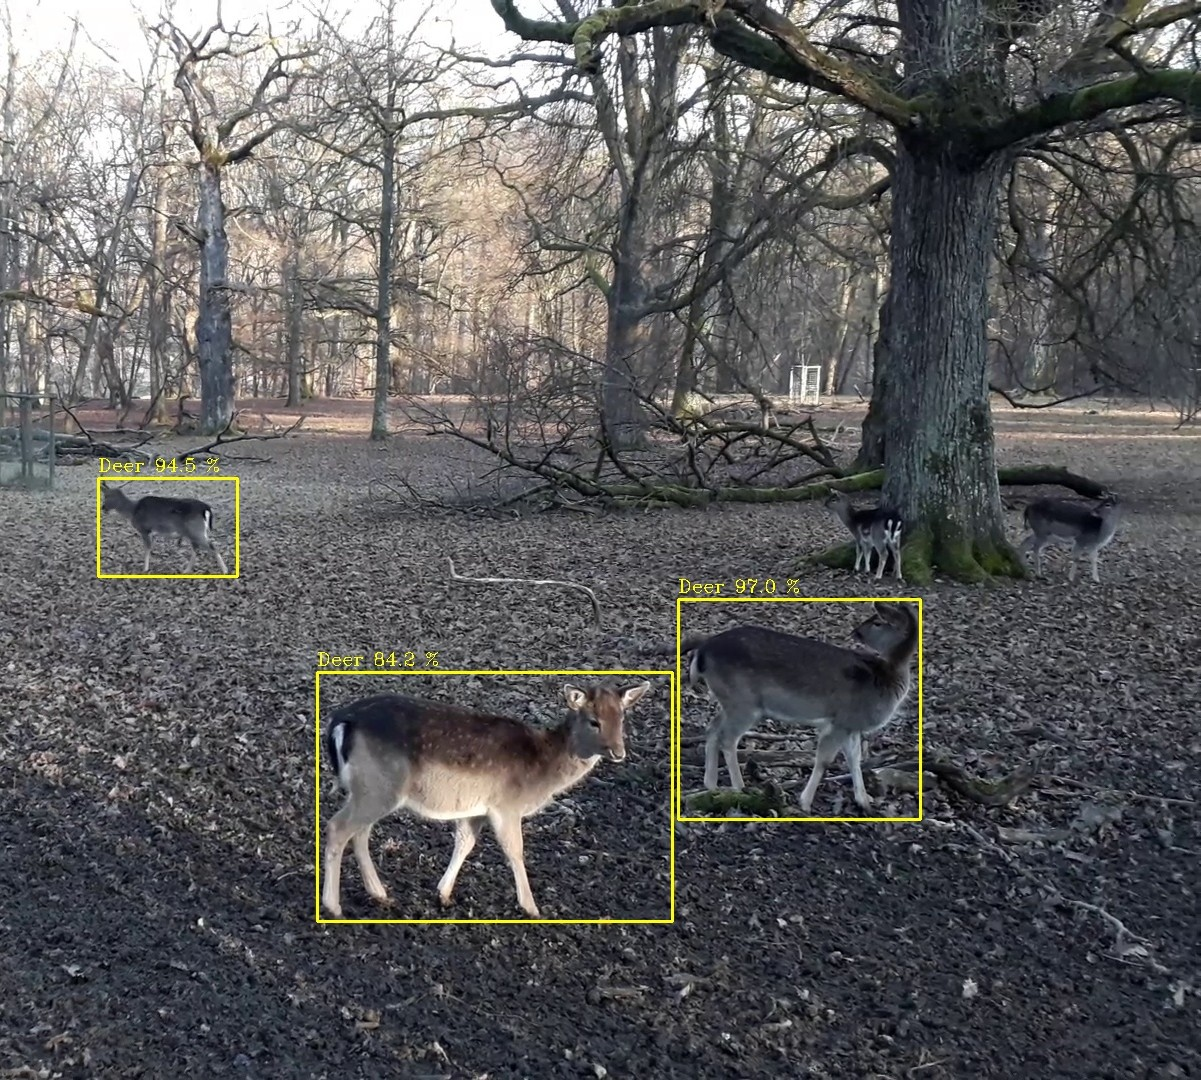
\includegraphics[width=0.9\textwidth]{model_compare_handy_faster_rcnn_inception_v2_early_stopping_ohne_aug.jpg}
  \captionof{figure}{Faster R-CNN + Early Stopping}
  \label{fig:infer_res_rcnn_early_stopping}
\end{minipage}
\begin{minipage}{0.5\textwidth}
  \centering
  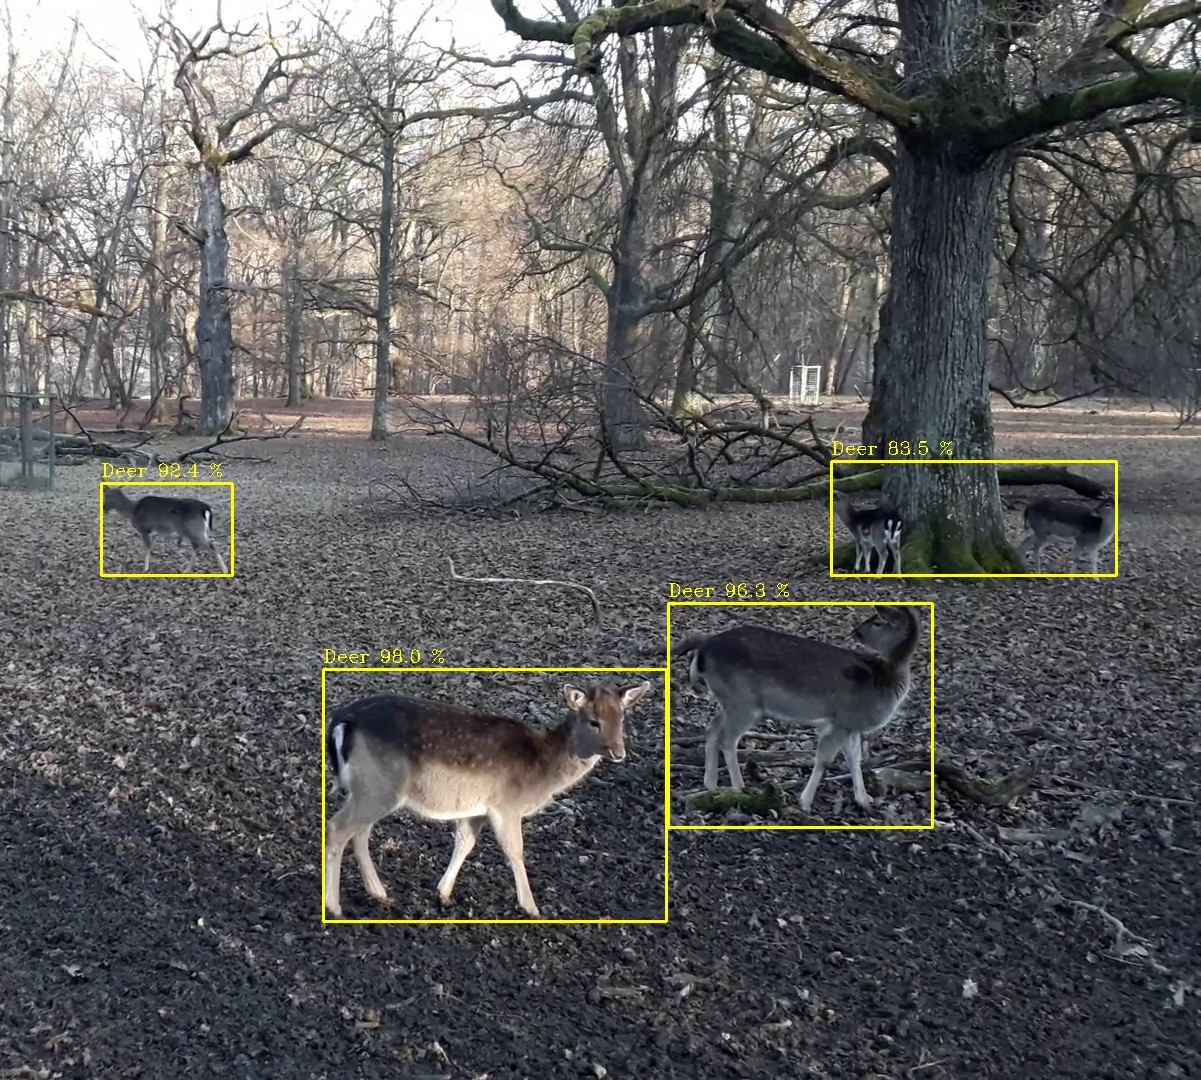
\includegraphics[width=0.9\textwidth]{model_compare_handy_faster_rcnn_inception_v2_early_stopping.jpg}
  \captionof{figure}{Faster R-CNN + Aug}
  \label{fig:infer_rest_rcnn_aug}
\end{minipage}
\vspace{1cm}

Auch hier fällt auf das besonders bei Tieren auf 
kleineren Skalen die Faster R-CNN Architekturen
bessere Ergebnisse liefern konnten.



\subsubsection{iWildCam}

Aus der von Kaggle veröffentlichten \textit{iWildCam 2019 Competition}
wurden die Klassen, welche sich mit für das Training verwendeten  
überschnitten, heruntergeladen und testweise inferiert.

Die Bilder stellen dabei aufnahmen von Wildtier Kameras aus 
dem Süd- und Nordwesten Amerikas dar, welche aus 
der iNaturalist Datenbank und von Microsoft DatAirSim stammen.
\cite{beery2019iwildcam}.

Darunter enthalten waren viele Nachtaufnahmen, welche wenig 
beleuchtet und mit Infraro Kameras aufgenommen und in Graustufen 
dargestellt waren.


Da die Ergebnisse bei allen vier Modellen deutlich schlechter
als bei dem Openimages Datensatz und den eigenen Bildern waren, 
wurde, versucht diese durch weitere Optimierungen zu verbessern.



%----------------- SECTION: optimierung ---------------------
\section{Optimierungen: Faster R-CNN}\label{sec:optimierung_faster_rcnn}

Als Ausgangslage zur Verbesserung der Ergebnisse, diente 
nun das Faster R-CNN mit, augmentiertem Datensatz, welches 
im vorherigen Abschnitt die besten Resultate erzielte.

Zunächst werden auch in diesem Abschnitt die Ergebnisse der 
anhand der Evaluierungsmetriken und Trainingsverläufen 
der Tensorboard Visualisierungen aufgeführt und anschließend
anhand testweise ausgeführter Inferenzen weiter verglichen.




\subsection{Verschiedene Augmentierungen}

Der erste Ansatz war, das Faster R-CNN mit 
variierendem Augmentierungsgrad der Daten für insgesamt
mehr Iterationen (500k statt 200k) zu trainieren 

Dabei wurde wieder das im Abschnitt \ref{subsec:augmentation} 
erläuterte Augmentierungsverfahren angewendetet, mit den variationen
\begin{enumerate}
  \item nur eine (zufällige) Augmentierung pro Bild, anstatt zwei
  \item 4000 Bilder pro Klasse anstatt 3000 generieren
\end{enumerate}

Die Trainingsergebnisse für 500k Iterationen sind anhand der 
Trainingsverläufe von Loss und mAP in den Plots
\ref{plot:map_diff_aug} und \ref{plot:loss_diff_aug} dargestellt.

\vspace{1cm}

\begin{minipage}{0.5\textwidth}
  \centering
  \def\svgwidth{0.9\textwidth}
  \input{Bilder/plots/diff_aug_map.pdf_tex}
  \captionof{figure}{mAP}
  \label{plot:map_diff_aug}
\end{minipage}
\begin{minipage}{0.5\textwidth}
  \centering
  \def\svgwidth{0.9\textwidth}
  \input{Bilder/plots/diff_aug_loss.pdf_tex}
  \captionof{figure}{Loss}
  \label{plot:loss_diff_aug}
\end{minipage}

% Legende
% orange: FF7043
% blue  : 0077BB
% red   : CC3311
\begin{table}[htb]
  \centering
  \begin{tabular}{m{0.1\textwidth}<{\centering}m{0.2\textwidth}<{\centering}m{0.2\textwidth}<{\centering}}
    $\color[HTML]{CC3311}\medbullet$  1 je bild & $\color[HTML]{FF7043}\medbullet$  3000 samples & $\color[HTML]{0077BB}\medbullet$  4000 samples
  \end{tabular}    
\end{table}

Aufgrund des länger durchgeführten Trainings ist bei allen Konfigureationen
im, gegensatz zu den Ergebnissen des vorherigen Abschnitts, Overfitting 
zu erkennen.

Dieses fällt, wie zu erwarten war, bei den weniger  
augmentierten Datensätzen stärker aus, welche auf der 
anderen Seite einen besseren mAP Wert erreichen konnten.

Welche Metrik sich positiver auf des Inferenzergebnis auswirkt 
soll über die Testinferenz, ausgeführt 
auf den iWildCam Datensatz, herausefunden werden.


\vspace{1cm}
\begin{minipage}{0.333\textwidth}
  \centering
  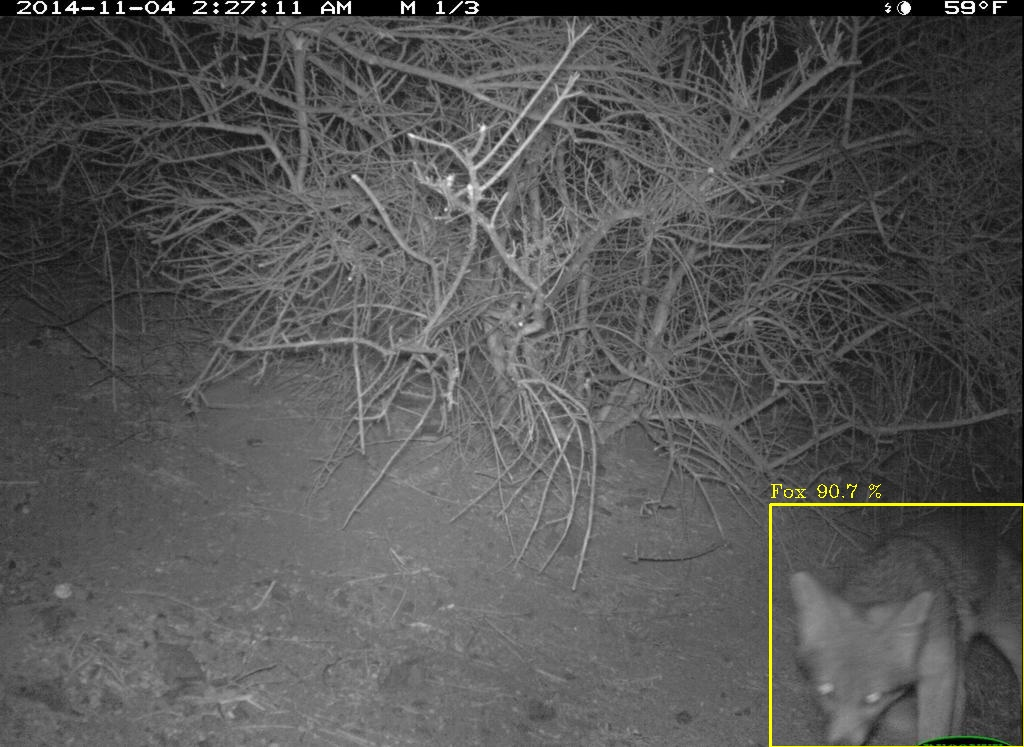
\includegraphics[width=\textwidth]{infer_images/iWildCam/fox/cut/59df5ee1-23d2-11e8-a6a3-ec086b02610b_faster_rcnn_inception_v2_3000.jpg}
  \captionof{figure}{3000 Samples}
  \label{fig:infer_res_3000}
\end{minipage}
\begin{minipage}{0.333\textwidth}
  \centering
  \label{fig:infer_res_4000}
  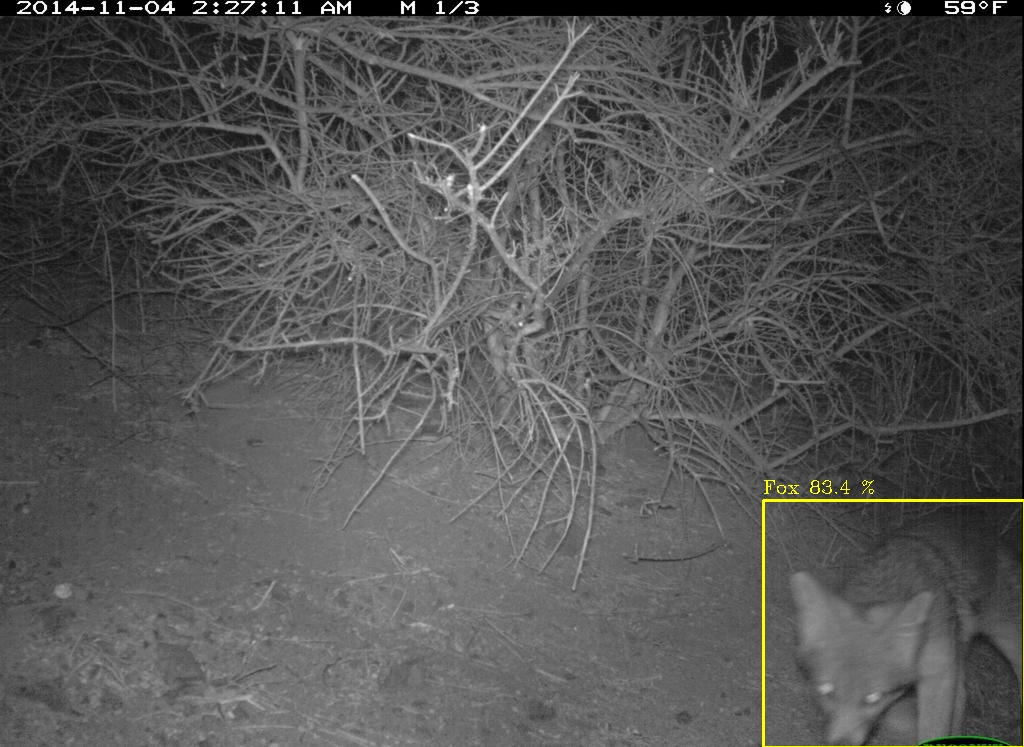
\includegraphics[width=\textwidth]{iWildCam/fox/cut/59df5ee1-23d2-11e8-a6a3-ec086b02610b_faster_rcnn_inception_v2_4000.jpg}
  \captionof{figure}{4000 Samples}
\end{minipage}
\begin{minipage}{0.333\textwidth}
  \centering
  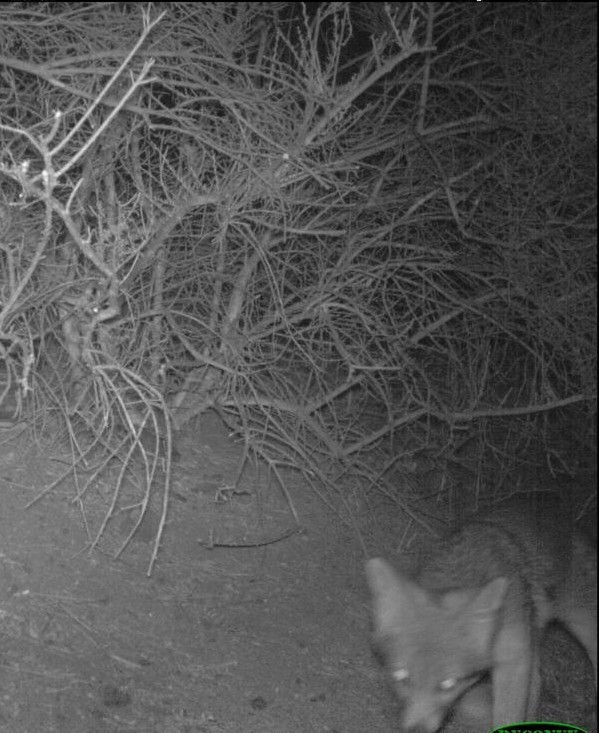
\includegraphics[width=\textwidth]{iWildCam/fox/cut/59df5ee1-23d2-11e8-a6a3-ec086b02610b_faster_rcnn_inception_v2_less_aug.jpg}
  \captionof{figure}{50\% Augment}
  \label{fig:infer_rest_05}
\end{minipage}
\vspace{1cm}

Abbildung \ref{fig:infer_res_3000} bis \ref{fig:infer_rest_05}
zeigen beispielhaft die Inferenz ergebnisse.
Weniger stark augmentierte Daten haben bei dem zum original 
Datensetz recht verschiedenen iWildCam Datensatz den effekt, 
das die Tiere schlechter bis gar nicht mehr erkannt wurden gehabt.



\subsection{Verschiedene Regularisierungen}

Um das trotz Augmentierung zu stande kommende Overfitting zu 
vermeiden, wurden nun zusätzlich die L2 Regularisierung angewendet.
Diese soll wie in den Grundlagen (\ref{subsec:validation}) beschrieben, 
durch anfügen der aufsummierten Geweichte an die Loss Funktion, 
die Überanpassugne reduzieren.

In der Konfigurationsdatei des Fater R-CNN kann dies durch setzten eines 
bestimmten Parameters für sowohl die erste Stufe des Netzes, 
dem RPN (Region Proposal Network), als auch für die zweite Stufe,
dem Klassifikationsmodell, seperat eingestellt werden.


Ebenso lassen sich die beiden Losskurven, aus denen sich 
beim Faster R-CNN der gesammt Loss zusammensetz,
seperat anzeigen was in den 
Plots \ref{plot:aug_l2_classifier_loss}
und \ref{plot:aug_l2_rpn_loss} dargestellt ist.

Durch die getrennte beobachtung der Loss Kurven ließ sich 
feststellen, dass Overfitting nur  beim Loss des RPNs 
stattfindet, weshalb der Parameter für die L2 Regulierung 
dann nur für die erste Stufe mit einem Faktor von
$\lambda = 0.001$ gesetzt.

Vergleicht man wieder die wieder die Losskurven, ist deutlich zu 
erkennen das sich das Overfitting im Regoin Proposal Network 
reduzieren ließ \ref{plot:aug_l2_rpn_loss}, wodurch sich 
auch der gesammt Loss verbesserte (Abbildung\ref{plot:aug_l2_total_loss}).

Auch hier ging die Verbesserung des Loss Wertes mit einer
leichten Verschlechterung des mAP einher, wie in 
\ref{plot:aug_l2_mAP} zu erkennen ist.



\vspace{1cm}
\begin{minipage}{0.5\textwidth}
  \centering
  \def\svgwidth{0.9\textwidth}
  \input{Bilder/plots/aug_l2_mAP.pdf_tex}
  \captionof{figure}{mAP}
  \label{plot:aug_l2_mAP}
\end{minipage}
\begin{minipage}{0.5\textwidth}
  \centering
  \def\svgwidth{0.9\textwidth}
  \input{Bilder/plots/aug_l2_total_loss.pdf_tex}
  \captionof{figure}{Total Loss}
  \label{plot:aug_l2_total_loss}
\end{minipage}
\\[1cm]
\begin{minipage}{0.5\textwidth}
  \centering
  \def\svgwidth{0.9\textwidth}
  \input{Bilder/plots/aug_l2_classifier_loss.pdf_tex}
  \captionof{figure}{Classifier Loss}
  \label{plot:aug_l2_classifier_loss}
\end{minipage}
\begin{minipage}{0.5\textwidth}
  \centering
  \def\svgwidth{0.9\textwidth}
  \input{Bilder/plots/aug_l2_rpn_loss.pdf_tex}
  \captionof{figure}{RPN Loss}
  \label{plot:aug_l2_rpn_loss}
\end{minipage}
\begin{table}[htb]
  \centering
  \begin{tabular}{m{0.3\textwidth}<{\centering}m{0.4\textwidth}<{\centering}}
    $\color[HTML]{CC3311}\medbullet$  nur Augmentierung & $\color[HTML]{0077BB}\medbullet$  Augmentierung+L2 Regulierung
  \end{tabular}    
\end{table}

\vspace{1cm}

Um die Auswirkung der in den Trainingsverläufen 
zu erkennenden Effekten zu überprüfen, wurd hier 
nun auch wieder die Inferenz auf die drei Testdatensetze 
ausgeführt.
Beispielhaft, sind Ergebnisse davon für eigene Bilder 
in den Abbildungen \ref{fig:test_infer_normal_aug}
und \ref{fig:test_infer_aug_plus_l2} dargestellt.


\vspace{1cm}
\begin{minipage}{0.5\textwidth}
  \centering
  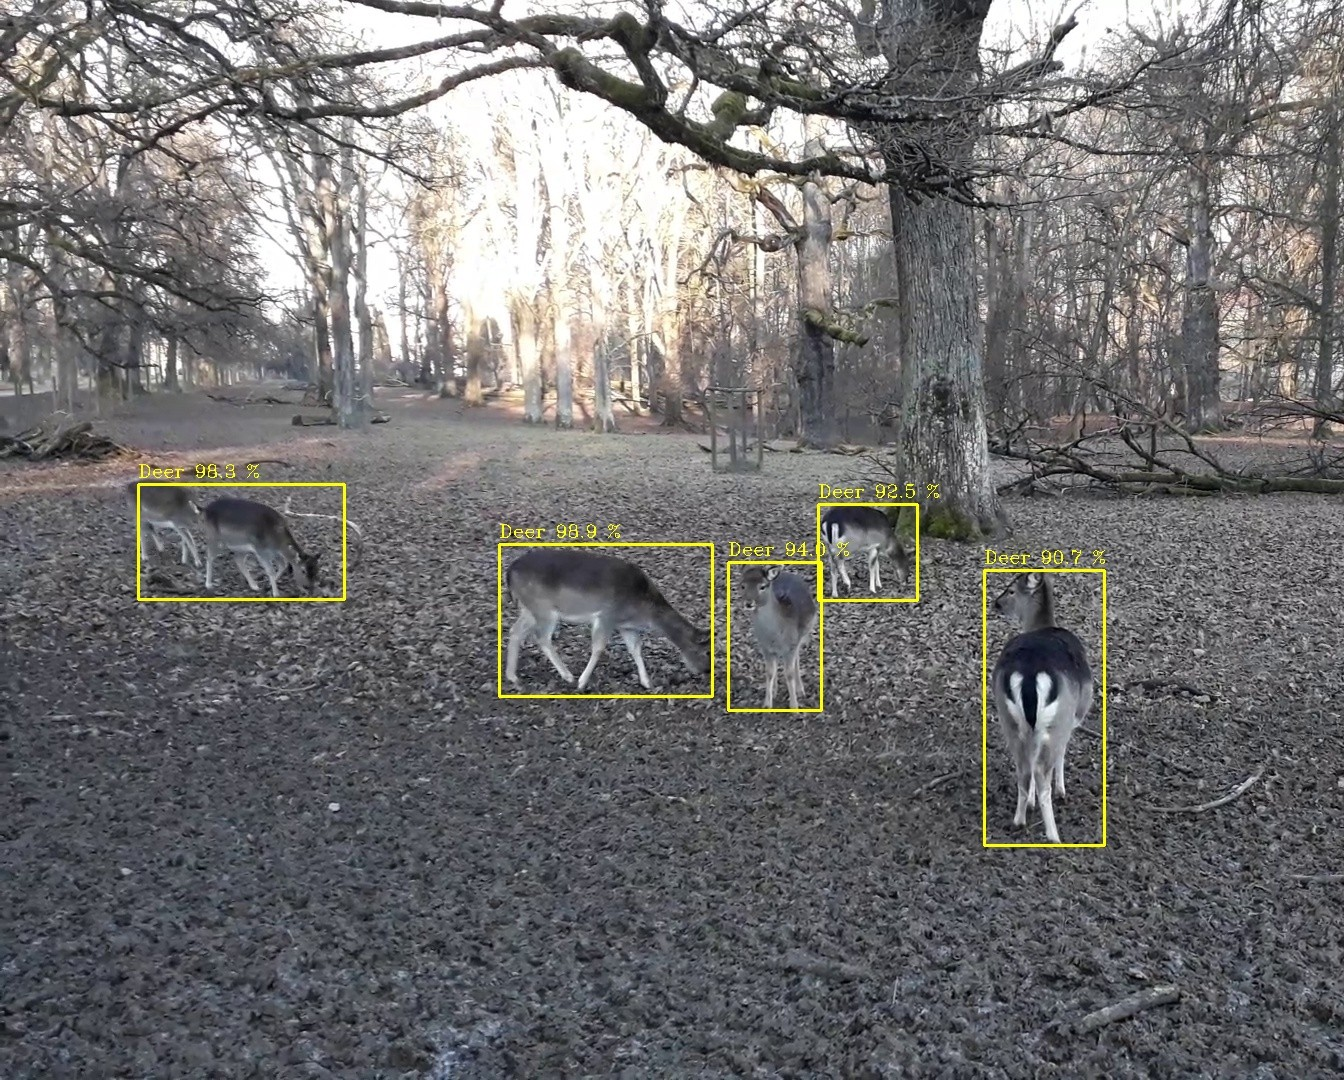
\includegraphics[width=0.95\textwidth]{eigene/20191229_145616_frame_20_faster_rcnn_inception_v2_3000.jpg}
  \captionof{figure}{}
  \label{fig:test_infer_normal_aug}
\end{minipage}
\begin{minipage}{0.5\textwidth}
  \centering
  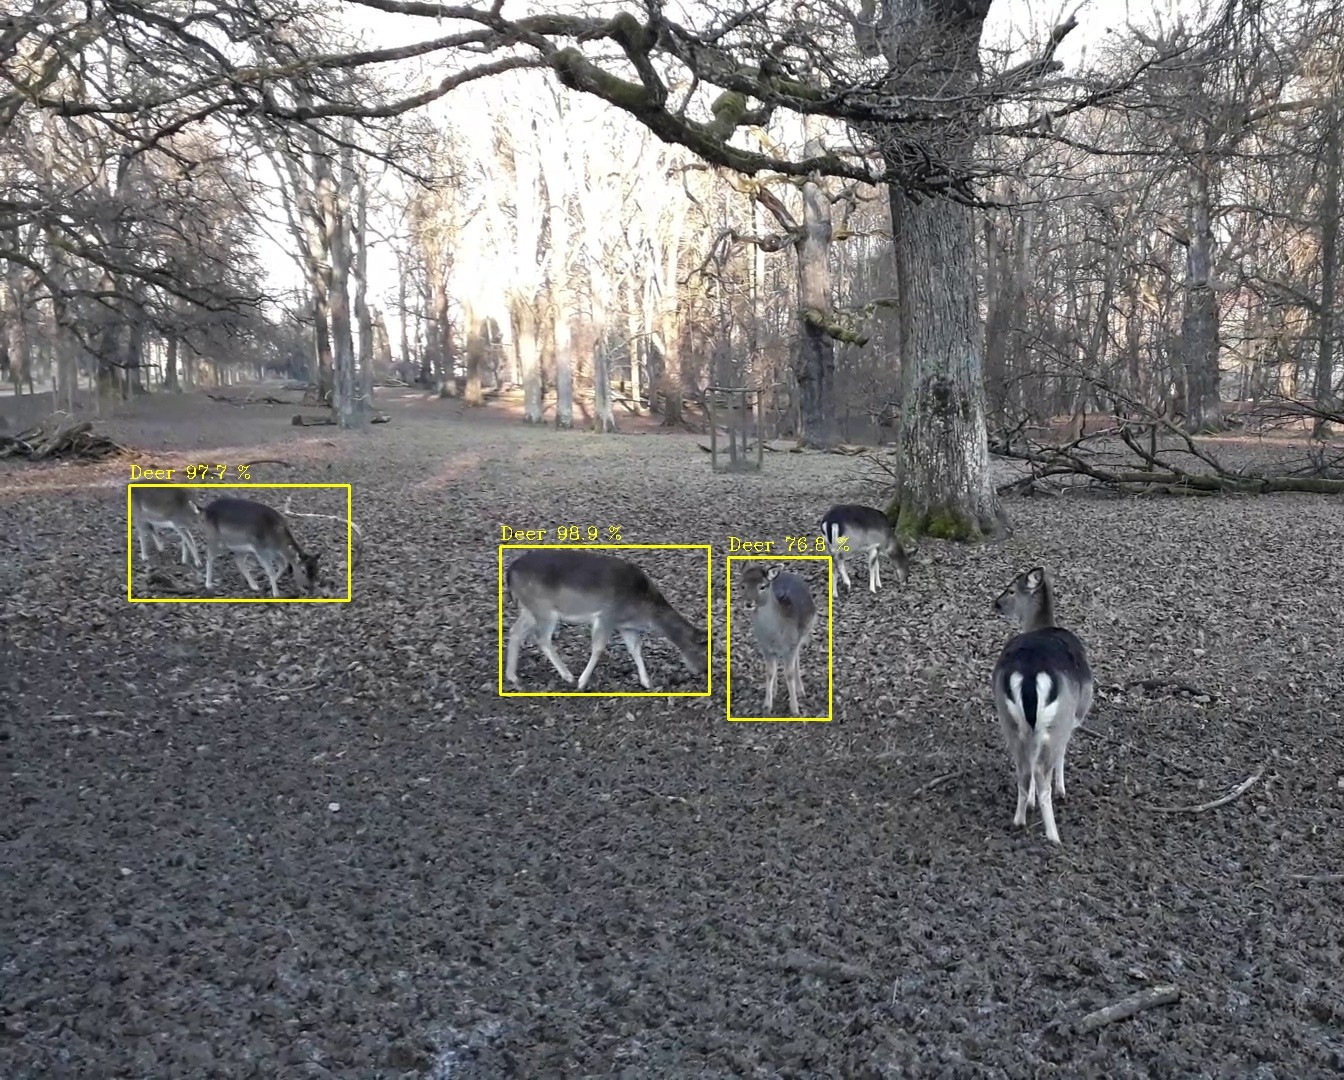
\includegraphics[width=0.95\textwidth]{eigene/20191229_145616_frame_20_faster_rcnn_inception_v2_l2.jpg}
  \captionof{figure}{}
  \label{fig:test_infer_aug_plus_l2}
\end{minipage}
\vspace{1cm}

Daraus ergab sich, das eine L2 Regulierung der Modelle 
in den meisten Fällen keinen Einfluss auf die Ergebnisse hatte,
falls doch fürte sie tendenziell eher zu einer Verschlechterung.


Weitere angewendete Regularisierungen, die jedoch 
auch zu keiner nennenswerten Veränderung des Trainingsergebnisses 
führten ware Dropout und L2 mit $\lambda = 0,02$ und sind in 
Tabelle \ref{table:reg} zusammen mit den anderen Ergebnissen dargestellt.

\vspace{1cm}
\begin{table}[htb]
  \centering
  \begin{tabular}{m{0.35\textwidth}|m{0.25\textwidth}<{\centering}m{0.25\textwidth}<{\centering}}
  \hline
                    & mAP  & Loss  \\ \hline\hline
  Augmentierung (50\%) &  0,72    &    0,76   \\
   + L2 Reg ($\lambda = 0,001$)            &   0,71     & 0,75       \\\hline
  Augmentierung (normal)     & 0,7  & 0,74            \\
  + Dropout          & 0,7  & 0,73            \\
  + L2 Reg. ($\lambda = 0,001$)    & 0,7  & 0,69            \\
  + L2 Reg ($\lambda = 0,002$)    & 0,69 & 0,7             \\ \hline
  Augmentierung (4000 Samples) &0,7&0,71\\\hline
  \end{tabular}
  \caption{Regularisierungen}
  \label{table:reg}
\end{table}
\vspace{1cm}


Aus den Ergebnissen lässt sich schließen, dass die Art
der Aufbereitung der Daten den größeren Einfluss auf das Ergebniss haben
und durch Einstellung der Hyperparameter wenn überhaupt 
noch Finetuning betrieben werden kann.



\section{Inferenz zeit}\label{sec:infertime}

Neben der Genauigkeit war die Ausführungszeit welche ein Model für die 
Inferenz benötigt, ein weiteres Kriterium für die Auswahl des zu 
verwendenen Modells.
Einer der Faktoren, der die Inferenzzeit beeinflusst, ist die 
verwendete Hardware sowie Library.
Die Hardware war mit dem Neural Compute Stick 2 festgelegt, als 
Library kamen dabei OpenCV oder OpenVino in Frage, wobei
mit OpenVino die möglichkeit 
zur asynchronen Inferenzausführung sowie mehreren Inferenz Requests besteht,
wodurch sich die Inferenzzeit optimieren ließ.

Ein weiter Faktor ist die Komplexität der CNNs und die zur 
Objekterkennung verwendeten Architektur.

Üblicherweise sind Komplexere Modelle wie Faster R-CNN zwar genauer, 
jedoch auch langsamer.

Um den Effekt, den die drei unterschiedlichen 
für das Training verwendeten Varianten SSD + MobilenetV2, 
SSD + InceptionV2 und Faster R-CNN + InceptionV2 auf die Inferenzzeit
haben zu Untersuchen, wurden diese durch Messugen der FPS 
verglichen.

Dabei wurde die Asynchrone Inferenz mit unterschiedlicher Anzahl 
an Inferenz Requests verwendet, weshalb in diesem Abschnitt 
zunächst die Funktionsweise der Asynchronen Inferenzausfürung 
mit OpenVino erklärt wird.


\subsection{Asychrone Inferenz}

Wird die Inferenz im Synchronen Modus ausgeführt, kann immer
nur entweder inferiert oder 
die Bilddaten vor- bzw. nachverarbeitet werden.

Vorverarbeitung der Bilder beeinhaltet dabei 
z.B. die Umwandlung des von der Kamera gelieferten 
Bildformats in das für das jeweilige Model richtige 
Input Format.
Die Nachbereitung bezieht sich auf das verarbeiten 
der Inferenz Ergebnisse in der Anwendung.


Die implementierung in OpenVino 
erfolgt dementsprechend Sequentiell, wie 
im Allgorithmus \ref{code:sync} dargestellt ist.


Anhand des zeitlichen Ablaufs, welcher in Abbildung \ref{fig:sync}
zur veranschaulichung abgebildet ist, sind die Abschnitte, 
in denen keine Inferez stattfindet gut zu erkennen.


\vspace{1cm}
\begin{minipage}{0.1\textwidth}
  \hfill
\end{minipage}
\begin{minipage}{0.5\textwidth}
  \begin{algorithm}[H]
    \caption{Synchrone Inferenz}
    \label{code:sync}
    \begin{algorithmic}
    \WHILE{\TRUE}
        \STATE capture FRAME
        \STATE preprocess CURRENT InferRequest
        \STATE \textbf{start} CURRENT InferRequest
        \STATE \textbf{wait} for CURRENT InferRequest
        \STATE process CURRENT result
    \ENDWHILE
    \end{algorithmic}
  \end{algorithm}  
\end{minipage}
\begin{minipage}{0.4\textwidth}
  \centering
  \vspace{1cm}
  \def\svgwidth{0.5\textwidth}
  \input{Bilder/sy_asy_legend.pdf_tex}
\end{minipage}

\vspace{1cm}
\begin{figure}[H]
  \centering
  \def\svgwidth{0.9\textwidth}
  %\tikzset{
    desicion/.style={
        diamond,
        draw,
        text width=4em,
        text badly centered,
        inner sep=0pt
    },
    block/.style={
        rectangle,
        draw,
        text width=5em,
        text height=1em,
        text centered
    },
    arrow/.style={
        draw,
        >=latex,
        ->
    }
}


\begin{tikzpicture}

    \node(infer1) [block] {infer1};
    \draw[arrow] (0,-1em) -- (10,-1em);
    % \node (A) [desicion] {entschei\\dung};
    % \node (B) [block, below of=A, node distance=5cm, text width=5em] {bock};
    % \node (C) [block, right of=A, node distance=5cm] {noch ein\\bock};


    % \draw[arrow] (A) --  node [left, fill=white] {yes} (B);
    % \draw[arrow] (A) -- node [below, near end] {crap} (C); 
    % \draw[arrow] (B) -| node [near start, fill=white] {yes} (C);

\end{tikzpicture}

  \input{Bilder/sync_infer.pdf_tex}
  \caption{}
  \label{fig:sync}
\end{figure}


Da die inferenz auf dem Myriad Chip des Neural Compute Sticks
und nicht auf dem ausführenden Pc oder Raspberry läuft,
kann diese auch ungehindert parallel dazu ablaufen.

In OpenVino wird das mithilfe der Asynchronen Api erreicht, welche 
über einen bestimmten Funktionsaufruf in einem seperaten 
Thread gestatet wird.



Indem man vor Erhalt und Verarbeitung eines aktuellen 
Inferenz Ergebnisses den Request für den nächsten Durchlauf aufgibt, 
wie in Allgorithmus \ref{code:async} als Pseudocode dargestellt, 
kann der in Abbildung \ref{fig:async} dargestellte Zeitliche 
Ablauf erreicht werden.



\vspace{1cm}
\begin{minipage}{0.1\textwidth}
  \hfill
\end{minipage}
\begin{minipage}{0.5\textwidth}
  \begin{algorithm}[H]
    \caption{Asynchrone Inferenz}
    \label{code:async}
    \begin{algorithmic}
    \WHILE{\TRUE}
        \STATE capture FRAME
        \STATE preprocess NEXT InferRequest
        \STATE \textbf{start} NEXT InferRequest
          \STATE \textbf{wait} for CURRENT InferRequest
          \STATE process CURRENT result
          \STATE swap CURRENT and NEXT InferRequest
    \ENDWHILE
    \end{algorithmic}
  \end{algorithm}
\end{minipage}
\begin{minipage}{0.4\textwidth}
  \centering
  \vspace{1cm}
  \def\svgwidth{0.5\textwidth}
  \input{Bilder/sy_asy_legend.pdf_tex}
\end{minipage}

\vspace{1cm}

\begin{figure}[H]
  \centering
  \def\svgwidth{0.9\textwidth}
  \input{Bilder/async_infer.pdf_tex}
  \caption{}
  \label{fig:async}
\end{figure}

Die hier mit \textit{Current} und \textit{Next} bezeichneten 
Inferenz Requests entsprechen den indices der jeweiligen Requests
und können belieb erweitert werden. Dadurch
wird erreicht, dass die Inferenz auf mehreren Threads 
parallel ausgeführt wird.
% https://docs.openvinotoolkit.org/2018_R5/_samples_object_detection_demo_ssd_async_README.html



\subsection{Vergleich der Modelle}

Mithilfe eines Python Scripts in welchem die Asynchrone Inferenz 
für eine variabel einstellbare Anzahl an inferenz Requests,
implementiert wurde, konnte für die drei Modelle die 
durchschnittliche Anzahl an Frames die pro Sekunge inferiert werden 
könenn ermittelt werden.

Diese wurde auf dem Raspberry Pi und dem Neural Compute Stick 
ausgeführt und liefert die in Tabelle \ref{table:infertime}
dargestellten Ergebnisse.

\vspace{1cm}
\begin{table}[htb]
  \centering
  \label{table:infertime}
  \begin{tabular}{m{0.25\textwidth}|m{0.1\textwidth}<{\centering}|m{0.1\textwidth}<{\centering}|m{0.1\textwidth}<{\centering}|m{0.1\textwidth}<{\centering}}
  \hline
  \multirow{2}{*}{Model} & \multicolumn{4}{c}{Asynchronge Inferenz Requests} \\ \cline{2-5} 
                         & 1           & 2          & 3          & 4          \\ \hline\hline
  SSD MobilenetV2        & 19,5           & 35,2          & 40,6          & 40,3          \\
  SSD InceptionV2        & 15,6           & 27,7          & 31,1          & 31,7          \\
  Faster R-CNN Incept.   & 0,63           & 0,67          & 0,75          & 0,74          \\ \hline
  \end{tabular}
  \caption{Vergleich Inferenz Zeiten Modelle}
\end{table}
\vspace{1cm}

Die asynchrone inferenz ausführung führte bei alle Modellen 
für bis zu 3 inferenz Requests zu besseren Ergebnissen.
Ein Unterschied in der benötigten Zeit macht sich besonders 
stark zwischen SSD Faster R-CNN Architekuren bemerkbar.
Für Real-Time Anwendungen kommen daher nur die mit SSD Trainierten 
Modelle in Frage. 
Ob und wie das Fater R-CNN trotz der recht langsamen Inferenzzeit 
für die Anwendung verwendet werden können, wird im nächstem Kapitel 
erläutert werden.

